\section{Dynamic Behavior Analysis}
\label{sec:dynamic_behavior}

This section analyzes the dynamic aspects of the Robotic Ultrasound System, focusing on runtime behavior, interaction patterns, and temporal characteristics that define system operation under various conditions.

\subsection{System Execution Flow}
\label{subsec:execution_flow}

The system's execution follows well-defined phases, each with specific responsibilities and performance characteristics.

\subsubsection{Initialization Phase}

During system startup, components are initialized in a specific order to ensure proper dependency resolution:

\begin{figure}[h]
\centering
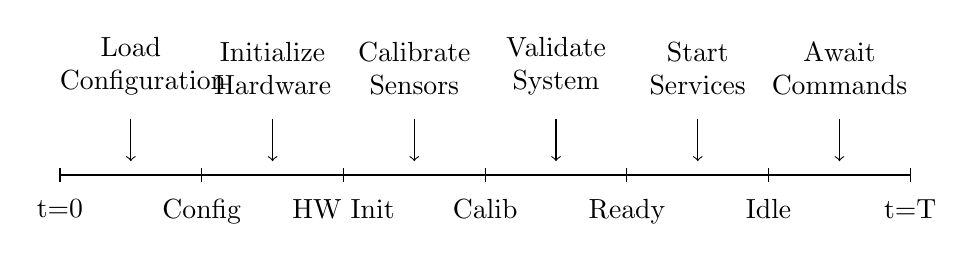
\begin{tikzpicture}[scale=0.9]
% Timeline
\draw[thick] (0,0) -- (12,0);
\foreach \x in {0,2,4,6,8,10,12}
    \draw (\x,0.1) -- (\x,-0.1);

% Labels
\node[below] at (0,-0.2) {t=0};
\node[below] at (2,-0.2) {Config};
\node[below] at (4,-0.2) {HW Init};
\node[below] at (6,-0.2) {Calib};
\node[below] at (8,-0.2) {Ready};
\node[below] at (10,-0.2) {Idle};
\node[below] at (12,-0.2) {t=T};

% Activities
\node[above, text width=1.8cm, align=center] at (1,1) {Load\\Configuration};
\node[above, text width=1.8cm, align=center] at (3,1) {Initialize\\Hardware};
\node[above, text width=1.8cm, align=center] at (5,1) {Calibrate\\Sensors};
\node[above, text width=1.8cm, align=center] at (7,1) {Validate\\System};
\node[above, text width=1.8cm, align=center] at (9,1) {Start\\Services};
\node[above, text width=1.8cm, align=center] at (11,1) {Await\\Commands};

% Arrows
\foreach \x in {1,3,5,7,9,11}
    \draw[->] (\x,0.8) -- (\x,0.2);

\end{tikzpicture}
\caption{System Initialization Timeline}
\label{fig:initialization_timeline}
\end{figure}

\begin{lstlisting}[language=C++, caption=System Initialization Sequence]
class SystemInitializer {
public:
    bool initialize() {
        try {
            // Phase 1: Configuration loading
            if (!loadConfiguration()) {
                log(ERROR, "Failed to load system configuration");
                return false;
            }
            
            // Phase 2: Hardware initialization
            if (!initializeHardware()) {
                log(ERROR, "Hardware initialization failed");
                return false;
            }
            
            // Phase 3: Sensor calibration
            if (!calibrateSensors()) {
                log(WARNING, "Sensor calibration incomplete");
                // Continue with degraded functionality
            }
            
            // Phase 4: System validation
            if (!validateSystem()) {
                log(ERROR, "System validation failed");
                return false;
            }
            
            // Phase 5: Service startup
            startServices();
            
            log(INFO, "System initialization completed successfully");
            return true;
            
        } catch (const std::exception& e) {
            log(ERROR, "Initialization exception: " + std::string(e.what()));
            return false;
        }
    }
    
private:
    bool loadConfiguration() {
        configManager_ = std::make_unique<ConfigurationManager>();
        return configManager_->loadFromFile("config/system.yaml");
    }
    
    bool initializeHardware() {
        hardwareManager_ = std::make_unique<HardwareManager>();
        return hardwareManager_->initializeAll();
    }
    
    bool calibrateSensors() {
        calibrationManager_ = std::make_unique<CalibrationManager>();
        return calibrationManager_->performAutoCalibration();
    }
    
    bool validateSystem() {
        validator_ = std::make_unique<SystemValidator>();
        return validator_->runDiagnostics();
    }
    
    void startServices() {
        serviceManager_ = std::make_unique<ServiceManager>();
        serviceManager_->startAllServices();
    }
};
\end{lstlisting}

\subsubsection{Operational Phase Transitions}

The system transitions between operational phases based on user commands and internal state changes:

\begin{figure}[h]
\centering
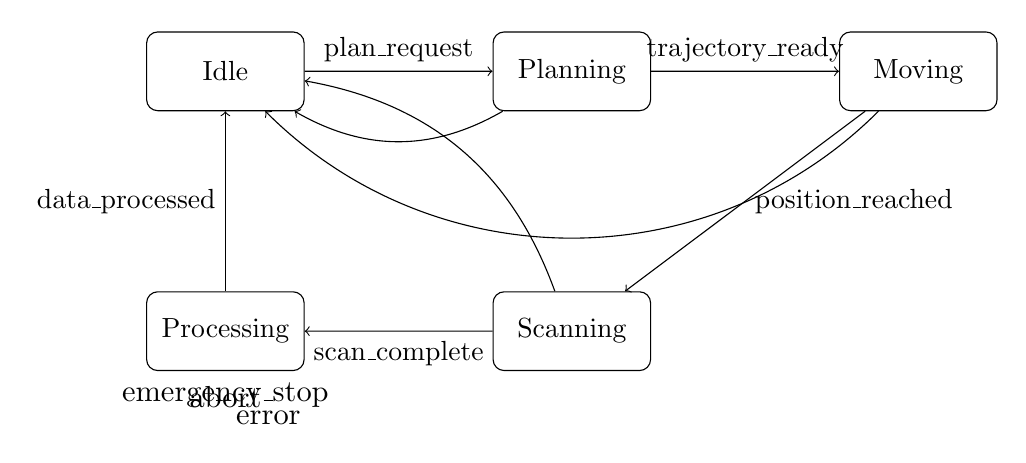
\begin{tikzpicture}[scale=1.1]
% States
\node[draw, rectangle, rounded corners, minimum width=2cm, minimum height=1cm] (idle) at (0,4) {Idle};
\node[draw, rectangle, rounded corners, minimum width=2cm, minimum height=1cm] (planning) at (4,4) {Planning};
\node[draw, rectangle, rounded corners, minimum width=2cm, minimum height=1cm] (moving) at (8,4) {Moving};
\node[draw, rectangle, rounded corners, minimum width=2cm, minimum height=1cm] (scanning) at (4,1) {Scanning};
\node[draw, rectangle, rounded corners, minimum width=2cm, minimum height=1cm] (processing) at (0,1) {Processing};

% Transitions
\draw[->] (idle) -- (planning) node[midway, above] {plan\_request};
\draw[->] (planning) -- (moving) node[midway, above] {trajectory\_ready};
\draw[->] (moving) -- (scanning) node[midway, right] {position\_reached};
\draw[->] (scanning) -- (processing) node[midway, below] {scan\_complete};
\draw[->] (processing) -- (idle) node[midway, left] {data\_processed};

% Emergency transitions
\draw[->] (planning) to[bend left=30] (idle) node[midway, above] {abort};
\draw[->] (moving) to[bend left=45] (idle) node[midway, above] {emergency\_stop};
\draw[->] (scanning) to[bend right=30] (idle) node[midway, right] {error};

\end{tikzpicture}
\caption{Operational Phase State Machine}
\label{fig:operational_phases}
\end{figure}

\subsection{Concurrency and Synchronization}
\label{subsec:concurrency}

The system employs sophisticated concurrency patterns to achieve real-time performance while maintaining data consistency.

\subsubsection{Thread Architecture}

\begin{figure}[h]
\centering
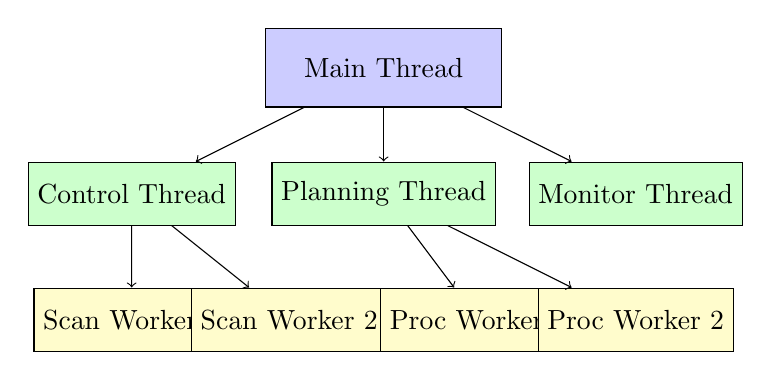
\begin{tikzpicture}[scale=0.8]
% Main thread
\node[draw, rectangle, minimum width=3cm, minimum height=1cm, fill=blue!20] (main) at (0,5) {Main Thread};

% Control threads
\node[draw, rectangle, minimum width=2.5cm, minimum height=0.8cm, fill=green!20] (control) at (-4,3) {Control Thread};
\node[draw, rectangle, minimum width=2.5cm, minimum height=0.8cm, fill=green!20] (planning) at (0,3) {Planning Thread};
\node[draw, rectangle, minimum width=2.5cm, minimum height=0.8cm, fill=green!20] (monitoring) at (4,3) {Monitor Thread};

% Worker threads
\node[draw, rectangle, minimum width=2cm, minimum height=0.8cm, fill=yellow!20] (scan1) at (-4,1) {Scan Worker 1};
\node[draw, rectangle, minimum width=2cm, minimum height=0.8cm, fill=yellow!20] (scan2) at (-1.5,1) {Scan Worker 2};
\node[draw, rectangle, minimum width=2cm, minimum height=0.8cm, fill=yellow!20] (proc1) at (1.5,1) {Proc Worker 1};
\node[draw, rectangle, minimum width=2cm, minimum height=0.8cm, fill=yellow!20] (proc2) at (4,1) {Proc Worker 2};

% Connections
\draw[->] (main) -- (control);
\draw[->] (main) -- (planning);
\draw[->] (main) -- (monitoring);
\draw[->] (control) -- (scan1);
\draw[->] (control) -- (scan2);
\draw[->] (planning) -- (proc1);
\draw[->] (planning) -- (proc2);

\end{tikzpicture}
\caption{Multi-threaded System Architecture}
\label{fig:thread_architecture}
\end{figure}

\subsubsection{Synchronization Mechanisms}

The system uses various synchronization primitives to coordinate between threads:

\begin{lstlisting}[language=C++, caption=Thread-Safe Data Management]
class ThreadSafeDataManager {
private:
    mutable std::shared_mutex dataMutex_;
    std::unordered_map<std::string, ScanData> scanDataCache_;
    
    // Condition variables for event coordination
    std::condition_variable dataReady_;
    std::condition_variable processingComplete_;
    
    // Atomic flags for state management
    std::atomic<bool> systemActive_{false};
    std::atomic<int> activeScanners_{0};
    
public:
    // Reader operations (multiple concurrent readers allowed)
    ScanData getScanData(const std::string& id) const {
        std::shared_lock<std::shared_mutex> lock(dataMutex_);
        auto it = scanDataCache_.find(id);
        return (it != scanDataCache_.end()) ? it->second : ScanData{};
    }
    
    // Writer operations (exclusive access required)
    void updateScanData(const std::string& id, const ScanData& data) {
        std::unique_lock<std::shared_mutex> lock(dataMutex_);
        scanDataCache_[id] = data;
        dataReady_.notify_all();
    }
    
    // Wait for data availability
    bool waitForData(const std::string& id, 
                    std::chrono::milliseconds timeout) {
        std::unique_lock<std::shared_mutex> lock(dataMutex_);
        return dataReady_.wait_for(lock, timeout, [this, &id]() {
            return scanDataCache_.find(id) != scanDataCache_.end();
        });
    }
    
    // Atomic operations for state management
    void setSystemActive(bool active) {
        systemActive_.store(active, std::memory_order_release);
    }
    
    bool isSystemActive() const {
        return systemActive_.load(std::memory_order_acquire);
    }
    
    void incrementActiveScanners() {
        activeScanners_.fetch_add(1, std::memory_order_acq_rel);
    }
    
    void decrementActiveScanners() {
        activeScanners_.fetch_sub(1, std::memory_order_acq_rel);
    }
    
    int getActiveScannerCount() const {
        return activeScanners_.load(std::memory_order_acquire);
    }
};
\end{lstlisting}

\subsection{Real-time Performance Analysis}
\label{subsec:realtime_performance}

The system's real-time characteristics are critical for safe and effective ultrasound operations.

\subsubsection{Timing Constraints}

\begin{table}[h]
\centering
\begin{tabular}{|l|c|c|c|c|}
\hline
\textbf{Operation} & \textbf{Target (ms)} & \textbf{Max (ms)} & \textbf{Typical (ms)} & \textbf{Priority} \\
\hline
Probe position update & 10 & 20 & 8 & High \\
Scan data acquisition & 50 & 100 & 45 & High \\
Trajectory planning & 500 & 1000 & 350 & Medium \\
Image processing & 200 & 500 & 180 & Medium \\
Safety monitoring & 5 & 10 & 3 & Critical \\
UI update & 100 & 200 & 80 & Low \\
\hline
\end{tabular}
\caption{System Timing Requirements}
\label{tab:timing_requirements}
\end{table}

\subsubsection{Deterministic Scheduling}

The system employs priority-based scheduling to meet real-time constraints:

\begin{lstlisting}[language=C++, caption=Real-time Task Scheduler]
class RealTimeScheduler {
public:
    enum class Priority {
        CRITICAL = 0,   // Safety monitoring, emergency stops
        HIGH = 1,       // Control loops, sensor updates
        MEDIUM = 2,     // Planning, processing
        LOW = 3         // UI, logging, housekeeping
    };
    
private:
    struct Task {
        std::function<void()> function;
        Priority priority;
        std::chrono::milliseconds period;
        std::chrono::steady_clock::time_point nextExecution;
        
        bool operator<(const Task& other) const {
            if (priority != other.priority)
                return priority > other.priority; // Lower enum value = higher priority
            return nextExecution > other.nextExecution;
        }
    };
    
    std::priority_queue<Task> taskQueue_;
    std::mutex queueMutex_;
    std::condition_variable taskAvailable_;
    std::atomic<bool> running_{false};
    
public:
    void scheduleTask(std::function<void()> task, Priority priority, 
                     std::chrono::milliseconds period) {
        std::lock_guard<std::mutex> lock(queueMutex_);
        Task newTask{
            std::move(task),
            priority,
            period,
            std::chrono::steady_clock::now() + period
        };
        taskQueue_.push(newTask);
        taskAvailable_.notify_one();
    }
    
    void executionLoop() {
        running_ = true;
        while (running_) {
            std::unique_lock<std::mutex> lock(queueMutex_);
            
            if (taskQueue_.empty()) {
                taskAvailable_.wait(lock);
                continue;
            }
            
            Task nextTask = taskQueue_.top();
            auto now = std::chrono::steady_clock::now();
            
            if (nextTask.nextExecution <= now) {
                taskQueue_.pop();
                lock.unlock();
                
                // Execute task with timing measurement
                auto startTime = std::chrono::high_resolution_clock::now();
                nextTask.function();
                auto endTime = std::chrono::high_resolution_clock::now();
                
                // Log timing violations
                auto executionTime = 
                    std::chrono::duration_cast<std::chrono::milliseconds>
                    (endTime - startTime);
                
                if (executionTime > nextTask.period) {
                    logTimingViolation(nextTask.priority, executionTime, 
                                     nextTask.period);
                }
                
                // Reschedule periodic task
                nextTask.nextExecution = now + nextTask.period;
                
                lock.lock();
                taskQueue_.push(nextTask);
            } else {
                // Wait until next task is due
                taskAvailable_.wait_until(lock, nextTask.nextExecution);
            }
        }
    }
    
private:
    void logTimingViolation(Priority priority, 
                          std::chrono::milliseconds actual,
                          std::chrono::milliseconds expected) {
        std::string priorityStr = priorityToString(priority);
        log(WARNING, "Timing violation in " + priorityStr + 
            " task: " + std::to_string(actual.count()) + "ms > " + 
            std::to_string(expected.count()) + "ms");
    }
};
\end{lstlisting}

\subsection{Error Handling and Recovery}
\label{subsec:error_handling}

The system implements comprehensive error handling mechanisms to ensure graceful degradation and recovery.

\subsubsection{Exception Hierarchy}

\begin{figure}[h]
\centering
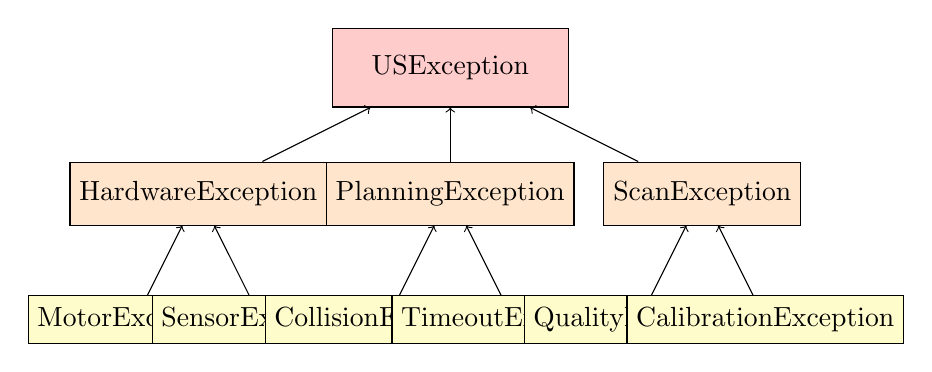
\begin{tikzpicture}[scale=0.8]
% Base exception
\node[draw, rectangle, minimum width=3cm, minimum height=1cm, fill=red!20] (base) at (0,4) {USException};

% Level 1 exceptions
\node[draw, rectangle, minimum width=2.5cm, minimum height=0.8cm, fill=orange!20] (hardware) at (-4,2) {HardwareException};
\node[draw, rectangle, minimum width=2.5cm, minimum height=0.8cm, fill=orange!20] (planning) at (0,2) {PlanningException};
\node[draw, rectangle, minimum width=2.5cm, minimum height=0.8cm, fill=orange!20] (scan) at (4,2) {ScanException};

% Level 2 exceptions
\node[draw, rectangle, minimum width=2cm, minimum height=0.6cm, fill=yellow!20] (motor) at (-5,0) {MotorException};
\node[draw, rectangle, minimum width=2cm, minimum height=0.6cm, fill=yellow!20] (sensor) at (-3,0) {SensorException};
\node[draw, rectangle, minimum width=2cm, minimum height=0.6cm, fill=yellow!20] (collision) at (-1,0) {CollisionException};
\node[draw, rectangle, minimum width=2cm, minimum height=0.6cm, fill=yellow!20] (timeout) at (1,0) {TimeoutException};
\node[draw, rectangle, minimum width=2cm, minimum height=0.6cm, fill=yellow!20] (quality) at (3,0) {QualityException};
\node[draw, rectangle, minimum width=2cm, minimum height=0.6cm, fill=yellow!20] (calibration) at (5,0) {CalibrationException};

% Inheritance relationships
\draw[->] (hardware) -- (base);
\draw[->] (planning) -- (base);
\draw[->] (scan) -- (base);

\draw[->] (motor) -- (hardware);
\draw[->] (sensor) -- (hardware);
\draw[->] (collision) -- (planning);
\draw[->] (timeout) -- (planning);
\draw[->] (quality) -- (scan);
\draw[->] (calibration) -- (scan);

\end{tikzpicture}
\caption{Exception Class Hierarchy}
\label{fig:exception_hierarchy}
\end{figure}

\subsubsection{Recovery Strategies}

\begin{lstlisting}[language=C++, caption=Error Recovery Implementation]
class ErrorRecoveryManager {
public:
    enum class RecoveryAction {
        RETRY,
        FALLBACK,
        ABORT,
        RESTART_COMPONENT,
        EMERGENCY_STOP
    };
    
    struct RecoveryStrategy {
        std::function<bool()> condition;
        RecoveryAction action;
        int maxRetries;
        std::chrono::milliseconds retryDelay;
    };
    
private:
    std::unordered_map<std::string, std::vector<RecoveryStrategy>> strategies_;
    std::unordered_map<std::string, int> retryCounters_;
    
public:
    void registerStrategy(const std::string& exceptionType, 
                         const RecoveryStrategy& strategy) {
        strategies_[exceptionType].push_back(strategy);
    }
    
    bool handleException(const std::exception& e) {
        std::string exceptionType = typeid(e).name();
        
        auto strategiesIt = strategies_.find(exceptionType);
        if (strategiesIt == strategies_.end()) {
            // No specific strategy, use default
            return handleDefault(e);
        }
        
        for (const auto& strategy : strategiesIt->second) {
            if (strategy.condition && !strategy.condition()) {
                continue; // Strategy not applicable
            }
            
            switch (strategy.action) {
                case RecoveryAction::RETRY:
                    return handleRetry(exceptionType, strategy);
                    
                case RecoveryAction::FALLBACK:
                    return handleFallback(e);
                    
                case RecoveryAction::ABORT:
                    handleAbort(e);
                    return false;
                    
                case RecoveryAction::RESTART_COMPONENT:
                    return handleComponentRestart(e);
                    
                case RecoveryAction::EMERGENCY_STOP:
                    handleEmergencyStop(e);
                    return false;
            }
        }
        
        return false;
    }
    
private:
    bool handleRetry(const std::string& exceptionType, 
                    const RecoveryStrategy& strategy) {
        int& retryCount = retryCounters_[exceptionType];
        
        if (retryCount >= strategy.maxRetries) {
            log(ERROR, "Max retries exceeded for " + exceptionType);
            retryCount = 0; // Reset for future occurrences
            return false;
        }
        
        ++retryCount;
        log(INFO, "Retrying operation (attempt " + 
            std::to_string(retryCount) + "/" + 
            std::to_string(strategy.maxRetries) + ")");
        
        std::this_thread::sleep_for(strategy.retryDelay);
        return true;
    }
    
    bool handleFallback(const std::exception& e) {
        log(WARNING, "Activating fallback mode due to: " + 
            std::string(e.what()));
        // Implement fallback logic
        return activateFallbackMode();
    }
    
    void handleAbort(const std::exception& e) {
        log(ERROR, "Aborting current operation: " + std::string(e.what()));
        abortCurrentOperation();
    }
    
    bool handleComponentRestart(const std::exception& e) {
        log(WARNING, "Restarting component due to: " + 
            std::string(e.what()));
        return restartFailedComponent();
    }
    
    void handleEmergencyStop(const std::exception& e) {
        log(CRITICAL, "Emergency stop triggered: " + std::string(e.what()));
        triggerEmergencyStop();
    }
};
\end{lstlisting}

This dynamic behavior analysis demonstrates the system's sophisticated runtime characteristics, including proper concurrency management, real-time performance optimization, and robust error handling that ensures safe and reliable operation under various conditions.
